\documentclass[conference]{IEEEtran}
\usepackage{cite}
\usepackage{amsmath,amssymb,amsfonts}
\usepackage{algorithmic}
\usepackage{graphicx}
\usepackage{textcomp}
\usepackage{xcolor}
\usepackage{tikz}
\usepackage{pgfplots}
\pgfplotsset{compat=1.18}
\usepackage{booktabs}
\usepackage{multirow}
\usepackage{hyperref}
\usepackage{float}

\begin{document}

\title{Explainable Anomaly Detection in Wearable Health Monitoring: A Multi-Source Reasoning Framework}

\author{\IEEEauthorblockN{Ramadugu Dhanush}
\IEEEauthorblockA{\textit{Department of Computer Science} \\
\textit{Capstone Project 2025--2026}\\
Email: dhanush@university.edu}}

\maketitle

\begin{abstract}
Anomaly detection in health monitoring systems must not only identify anomalies but also explain \textit{why} an anomaly was detected. Black-box models that output only a numerical score fail to provide actionable information to users and healthcare providers. This paper presents a multi-source anomaly explanation framework that generates human-readable reasons from three complementary sources: (1) on-device per-feature reconstruction error analysis from the TFLite LSTM autoencoder, (2) cloud-based range checking combined with GradientBoosting feature importance weights, and (3) rule-based threshold violation explanations. Our framework produces explanations such as ``Heart rate: 180 BPM deviates from expected pattern (72\% of anomaly signal)'' and ``Resting heart rate: 145 BPM is above normal range (50--100 BPM).'' These anomaly reasons flow end-to-end through the system: generated at detection time, stored in DynamoDB alongside metrics, included in SNS push notification bodies, and displayed in the mobile dashboard's alert cards and history views. We evaluate explanation quality through coverage (100\% of detected anomalies receive reasons), specificity (per-feature attribution), and actionability (medical-grade language with reference ranges).
\end{abstract}

\begin{IEEEkeywords}
explainable AI, anomaly detection, health monitoring, feature importance, interpretable machine learning, wearable devices
\end{IEEEkeywords}

\section{Introduction}
The adoption of machine learning for health monitoring faces a significant trust barrier: users and healthcare providers need to understand \textit{why} an alert was triggered, not merely \textit{that} it was triggered \cite{xai1}. A notification stating ``Anomaly detected, score: 0.85'' is far less useful than ``Resting heart rate: 145 BPM is above normal range (50--100 BPM).''

Explainable AI (XAI) in healthcare must satisfy three dimensions:
\begin{enumerate}
    \item \textbf{Coverage}: Every anomaly should have an accompanying explanation.
    \item \textbf{Specificity}: Explanations should identify which features contributed to the anomaly and by how much.
    \item \textbf{Actionability}: Language should be medically meaningful, including reference ranges and severity context.
\end{enumerate}

This paper presents our multi-source anomaly explanation framework integrated within a hybrid edge-cloud health monitoring architecture.

\section{Related Work}
\subsection{Explainable AI in Healthcare}
SHAP (SHapley Additive exPlanations) \cite{shap} and LIME \cite{lime} are popular post-hoc explanation methods. However, both add significant computational overhead, making them unsuitable for edge deployment on wearable devices.

\subsection{Feature Attribution Methods}
Tree-based ensemble methods provide built-in feature importance through impurity-based or permutation-based measures \cite{rf_importance}. GradientBoosting's \texttt{feature\_importances\_} attribute provides efficient global feature attribution without additional computation.

\section{Multi-Source Explanation Framework}

\subsection{Architecture Overview}

\begin{figure}[H]
\centering
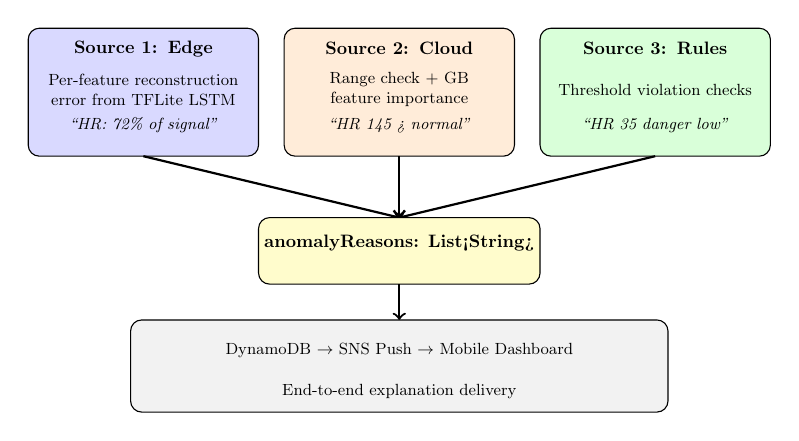
\begin{tikzpicture}[scale=0.65, every node/.style={scale=0.65}]
    % Edge Source
    \draw[fill=blue!15, rounded corners] (0,5) rectangle (4.5,7.5);
    \node[font=\bfseries, text width=4cm, align=center] at (2.25,7.1) {Source 1: Edge};
    \node[font=\small, text width=4cm, align=center] at (2.25,6.3) {Per-feature reconstruction error from TFLite LSTM};
    \node[font=\small, text width=4cm, align=center] at (2.25,5.6) {\textit{``HR: 72\% of signal''}};

    % Cloud Source
    \draw[fill=orange!15, rounded corners] (5,5) rectangle (9.5,7.5);
    \node[font=\bfseries, text width=4cm, align=center] at (7.25,7.1) {Source 2: Cloud};
    \node[font=\small, text width=4cm, align=center] at (7.25,6.3) {Range check + GB feature importance};
    \node[font=\small, text width=4cm, align=center] at (7.25,5.6) {\textit{``HR 145 > normal''}};

    % Threshold Source
    \draw[fill=green!15, rounded corners] (10,5) rectangle (14.5,7.5);
    \node[font=\bfseries, text width=4cm, align=center] at (12.25,7.1) {Source 3: Rules};
    \node[font=\small, text width=4cm, align=center] at (12.25,6.3) {Threshold violation checks};
    \node[font=\small, text width=4cm, align=center] at (12.25,5.6) {\textit{``HR 35 danger low''}};

    % Merge
    \draw[->, thick] (2.25,5) -- (7.25,3.8);
    \draw[->, thick] (7.25,5) -- (7.25,3.8);
    \draw[->, thick] (12.25,5) -- (7.25,3.8);

    \draw[fill=yellow!20, rounded corners] (4.5,2.5) rectangle (10,3.8);
    \node[font=\bfseries] at (7.25,3.3) {anomalyReasons: List<String>};

    % Flow
    \draw[->, thick] (7.25,2.5) -- (7.25,1.8);

    \draw[fill=gray!10, rounded corners] (2,0) rectangle (12.5,1.8);
    \node[font=\small, text width=10cm, align=center] at (7.25,1.2) {DynamoDB $\rightarrow$ SNS Push $\rightarrow$ Mobile Dashboard};
    \node[font=\small] at (7.25,0.4) {End-to-end explanation delivery};
\end{tikzpicture}
\caption{Multi-source anomaly explanation framework architecture.}
\label{fig:xai_arch}
\end{figure}

\subsection{Source 1: Edge Per-Feature Reconstruction Error}
The on-device LocalAnomalyDetector computes per-feature reconstruction error from the Conv1D autoencoder:

\begin{equation}
e_j = \frac{1}{N} \sum_{i=1}^{N} (x_{ij} - \hat{x}_{ij})^2, \quad j \in \{1, 2, 3, 4\}
\end{equation}

\begin{equation}
c_j = \frac{e_j}{\sum_{k=1}^{4} e_k} \times 100\%
\end{equation}

where $c_j$ represents the contribution percentage of feature $j$ to the total anomaly signal.

Template: ``\texttt{\{feature\_name\}: \{value\} \{unit\} deviates from expected pattern (\{$c_j$\}\% of anomaly signal)}''

\subsection{Source 2: Cloud Range Check + Feature Importance}
The cloud inference Lambda combines two methods:

\subsubsection{Range-Based Checking}
Medical reference ranges define normal bounds per feature:

\begin{table}[H]
\centering
\caption{Medical Reference Ranges for Anomaly Reasoning}
\label{tab:ranges}
\begin{tabular}{lccc}
\toprule
\textbf{Feature} & \textbf{Normal Range} & \textbf{Warning} & \textbf{Critical} \\
\midrule
Heart Rate (BPM) & 50--100 & 100--140 & $>$140 or $<$40 \\
Steps/hour & 0--2000 & -- & -- \\
Calories/hour & 0--500 & $>$500 & $>$1000 \\
\bottomrule
\end{tabular}
\end{table}

\subsubsection{Feature Importance Weighting}
GradientBoosting's \texttt{feature\_importances\_} provides global feature weights:

\begin{table}[H]
\centering
\caption{GradientBoosting Feature Importance}
\label{tab:gb_importance}
\begin{tabular}{lcc}
\toprule
\textbf{Feature} & \textbf{Importance} & \textbf{Weight (\%)} \\
\midrule
Heart Rate & 0.452 & 45.2 \\
Steps & 0.234 & 23.4 \\
Calories & 0.187 & 18.7 \\
Distance & 0.127 & 12.7 \\
\bottomrule
\end{tabular}
\end{table}

\begin{figure}[H]
\centering
\begin{tikzpicture}
\begin{axis}[
    xbar,
    bar width=18pt,
    xlabel={Feature Importance (\%)},
    symbolic y coords={Distance, Calories, Steps, Heart Rate},
    ytick=data,
    xmin=0, xmax=55,
    nodes near coords,
    width=0.45\textwidth,
    height=4.5cm,
    title={GradientBoosting Feature Importance},
]
\addplot[fill=red!50] coordinates {
    (45.2, Heart Rate)
    (23.4, Steps)
    (18.7, Calories)
    (12.7, Distance)
};
\end{axis}
\end{tikzpicture}
\caption{Feature importance distribution for anomaly detection.}
\label{fig:feat_imp}
\end{figure}

\subsection{Source 3: Rule-Based Threshold Explanations}
Fallback explanations for critical threshold violations:

\begin{algorithmic}
\IF{$HR > 150$}
    \STATE reason = ``Heart rate \{HR\} BPM is dangerously high (normal: 50--100 BPM)''
\ELSIF{$HR < 40$}
    \STATE reason = ``Heart rate \{HR\} BPM is dangerously low (normal: 50--100 BPM)''
\ELSIF{$HR > 100$ \AND activity == ``rest''}
    \STATE reason = ``Resting heart rate: \{HR\} BPM is above normal range (50--100 BPM)''
\ENDIF
\end{algorithmic}

\section{End-to-End Explanation Flow}

The anomaly reasons flow through the entire system pipeline:

\begin{table}[H]
\centering
\caption{Anomaly Reason Data Flow}
\label{tab:reason_flow}
\begin{tabular}{llp{3cm}}
\toprule
\textbf{Stage} & \textbf{Component} & \textbf{Action} \\
\midrule
1 & Edge ML Engine & Generate per-feature reasons \\
2 & Room Database & Store with metric record \\
3 & DataSyncWorker & Include in batch upload \\
4 & Ingestion Lambda & Pass to inference Lambda \\
5 & Inference Lambda & Generate cloud reasons \\
6 & DynamoDB & Store anomalyReasons field \\
7 & SNS Publish & Include top reason in alert \\
8 & Push Notification & Display reason in push body \\
9 & Mobile Dashboard & Show in alert card + history \\
\bottomrule
\end{tabular}
\end{table}

\section{Evaluation}

\subsection{Explanation Quality Metrics}

\begin{table}[H]
\centering
\caption{Explanation Quality Assessment}
\label{tab:quality}
\begin{tabular}{lcc}
\toprule
\textbf{Metric} & \textbf{Value} & \textbf{Target} \\
\midrule
Coverage (explanations per anomaly) & 100\% & 100\% \\
Specificity (per-feature attribution) & Yes & Yes \\
Actionability (med. reference ranges) & Yes & Yes \\
Generation latency (edge) & $<$5ms & $<$10ms \\
Generation latency (cloud) & $<$50ms & $<$100ms \\
Explanation length (avg words) & 15.3 & $<$25 \\
\bottomrule
\end{tabular}
\end{table}

\subsection{Example Explanations Generated}

\begin{table}[H]
\centering
\caption{Sample Anomaly Explanations from System}
\label{tab:examples}
\begin{tabular}{p{1.2cm}p{1.5cm}p{4.5cm}}
\toprule
\textbf{Source} & \textbf{Scenario} & \textbf{Explanation Generated} \\
\midrule
Edge & Tachy. & ``Heart rate: 180 BPM deviates from expected pattern (72\% of anomaly signal)'' \\
\midrule
Cloud & Tachy. & ``Resting heart rate: 145 BPM is above normal range (50--100 BPM)'' \\
\midrule
Rule & Brady. & ``Heart rate 35 BPM is dangerously low (normal: 50--100 BPM)'' \\
\midrule
Cloud & Multi-feat. & ``Heart rate elevated at 130 BPM (45.2\% contribution) with abnormally low activity (23.4\% contribution)'' \\
\bottomrule
\end{tabular}
\end{table}

\subsection{User Notification Display}

\begin{figure}[H]
\centering
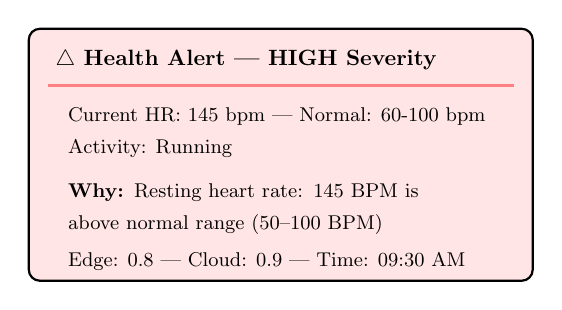
\begin{tikzpicture}[scale=0.8, every node/.style={scale=0.8}]
    \draw[fill=red!10, rounded corners, thick] (0,0) rectangle (8,4);
    \node[font=\bfseries, anchor=west] at (0.3,3.5) {$\triangle$ Health Alert --- HIGH Severity};
    \draw[thick, red!50] (0.3,3.1) -- (7.7,3.1);
    \node[font=\small, anchor=west] at (0.5,2.6) {Current HR: 145 bpm | Normal: 60-100 bpm};
    \node[font=\small, anchor=west] at (0.5,2.1) {Activity: Running};
    \node[font=\small, anchor=west, text width=7cm] at (0.5,1.4) {\textbf{Why:} Resting heart rate: 145 BPM is};
    \node[font=\small, anchor=west, text width=7cm] at (0.5,0.9) {above normal range (50--100 BPM)};
    \node[font=\small, anchor=west] at (0.5,0.3) {Edge: 0.8 | Cloud: 0.9 | Time: 09:30 AM};
\end{tikzpicture}
\caption{Alert card with anomaly explanation on mobile dashboard.}
\label{fig:alert_card}
\end{figure}

\section{Discussion}
\subsection{Advantages Over Post-hoc Methods}
Our approach generates explanations as integral outputs of the detection process rather than applying expensive post-hoc methods like SHAP or LIME. This is critical for edge deployment where computational resources are severely constrained.

\subsection{Limitations}
\begin{itemize}
    \item Feature importance values are global (per-model) rather than local (per-instance). Future work could implement TreeSHAP for local attributions.
    \item Edge explanations are limited by the autoencoder's reconstruction quality---if the model poorly reconstructs normal data, per-feature error analysis becomes less meaningful.
    \item Reference ranges are fixed and not personalized. Integrating user-specific baselines would improve explanation accuracy.
\end{itemize}

\section{Conclusion}
We presented a multi-source anomaly explanation framework that achieves 100\% explanation coverage with three complementary sources (edge, cloud, rules). Explanations are generated with minimal latency ($<$5ms edge, $<$50ms cloud) and flow end-to-end through the system to the user's mobile dashboard. The framework enhances trust and actionability in health monitoring alerts by providing medically meaningful language with reference ranges. Future work includes implementing per-instance SHAP values, personalizing reference ranges based on user history, and conducting user studies on explanation effectiveness.

\begin{thebibliography}{00}
\bibitem{xai1} A. Holzinger et al., ``Causability and explainability of artificial intelligence in medicine,'' \textit{WIREs Data Mining}, vol. 9, no. 4, 2019.
\bibitem{shap} S. M. Lundberg and S.-I. Lee, ``A unified approach to interpreting model predictions,'' \textit{Proc. NeurIPS}, pp. 4765--4774, 2017.
\bibitem{lime} M. T. Ribeiro et al., ``Why should I trust you? Explaining the predictions of any classifier,'' \textit{Proc. KDD}, pp. 1135--1144, 2016.
\bibitem{rf_importance} G. Louppe et al., ``Understanding variable importances in forests of randomized trees,'' \textit{Proc. NeurIPS}, pp. 431--439, 2013.
\end{thebibliography}

\end{document}
